\begin{figure}[ht]
	\centering
	\footnotesize


	\psfrag{x1}[l][l] {$x_1$}
	\psfrag{x2}[l][l] {$x_2$}

	\psfrag{r}[l][l] {$\rho(x,t)$}
	\psfrag{r1}[l][l] {$\rho(x_{1},t)$}
	\psfrag{r2}[l][l] {$\rho(x_{2},t)$}

	\psfrag{xst}[l][l] {$\displaystyle x=st\text{ or }t=\frac{x}{s}$}

	\psfrag{t}[l][l] {$t$}
	\psfrag{to}[l][l] {$t = 0$}
	\psfrag{ti}[l][l] {$t \rightarrow +\infty$}

	% \psfrag{i1}[c][c] {$\displaystyle I_{1} = \int_{0}^{+\infty}\int_{-\infty}^{+\infty} \left(\cdot\right)dxdt$}
	% \psfrag{i2}[c][c] {$\displaystyle I_{2} = \int_{-\infty}^{+\infty}\int_{0}^{+\infty} \left(\cdot\right)dtdx$}

	\psfrag{i1}[l][l] {$\displaystyle I_{1} = \int_{0}^{\mathscr{T}}\int_{-\infty}^{st} \left(\cdot\right)dxdt$}
	\psfrag{i2}[l][l] {$\displaystyle I_{2}
			=
			\int_{-\infty}^{0}\int_{0}^{+\infty} \left(\cdot\right)dtdx
			+
			\int_{0}^{+\infty}\int_{x/s}^{+\infty} \left(\cdot\right)dtdx
		$}

	\psfrag{x}[l][l] {$x$}
	\psfrag{yo}[l][l] {$x=0$}
	\psfrag{xl}[r][r] {$x\rightarrow -\infty$}
	\psfrag{xr}[l][l] {$x\rightarrow +\infty$}

	\psfrag{oh}[l][l] {$O$}
	\psfrag{id}[l][l] {$\text{Integration direction}$}

	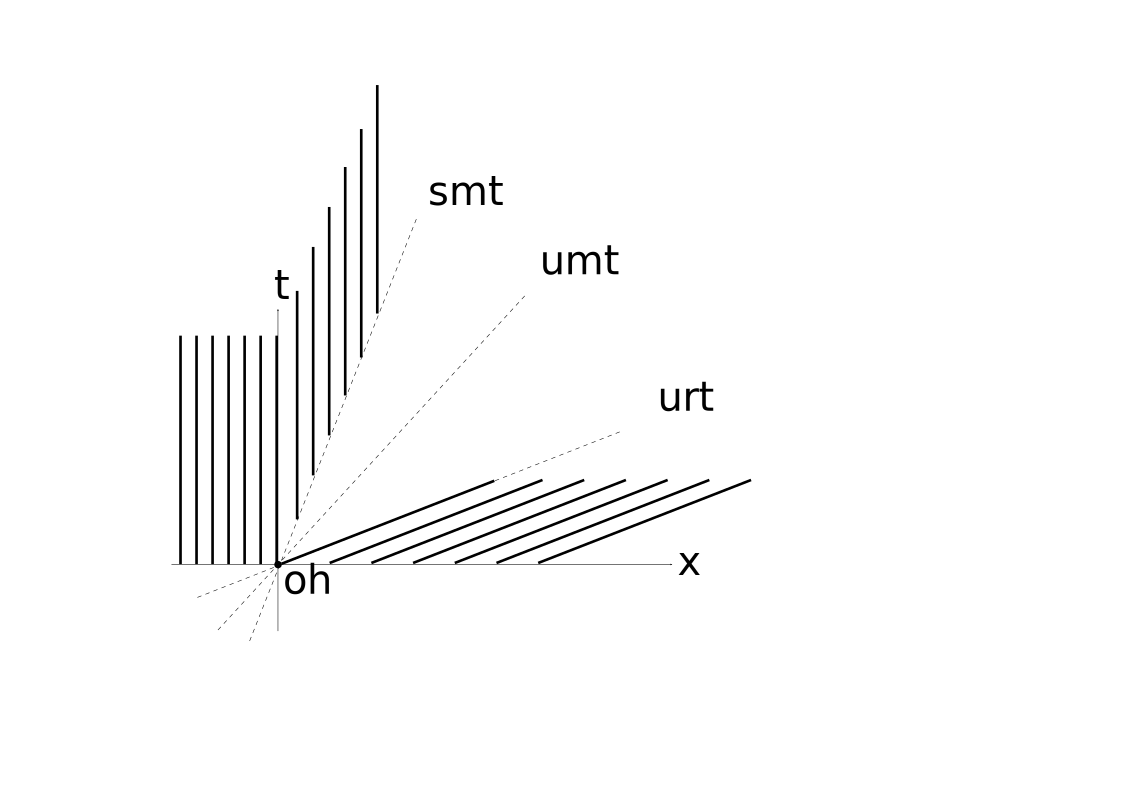
\includegraphics[width=0.9\textwidth]{rarefactionweaksol.eps}
	\caption{Difference of limits when swapping order of integrals is observed, i.e. the corresponding limits
		have to be adjusted in order to guarantee $I_{1} = I_{2}$.}
	\label{\LABEL}
\end{figure}
